\documentclass{beamer}
\mode<presentation>
{
\usepackage{dis-template}
}
\usepackage{textcomp}
\graphicspath{{slides/}} % TODO: eliminate this hack, necessary because scons builds at repository root

%---------------------------------------------------------------------
\titlepageinit{12}{Mechanical Tuning}{15 \& 16 Apr 2015 (Week 12)}
%---------------------------------------------------------------------
\begin{document}
%---------------------------------------------------------------------
\begin{frame}
\titlepage

\setcounter{tocdepth}{1}
\tableofcontents
\end{frame}

% LAB PREPARATION
% Have car to demo tuning procedure

%---------------------------------------------------------------------
\section{Introduction} % [?? mins]
%---------------------------------------------------------------------
\begin{frame}
\centering \huge Introduction
\end{frame}

\begin{frame}
\frametitle{Disclaimer}
\begin{columns}[t]
\column{0.646\textwidth}
  \begin{itemize}
    \item I'm not a mechanical engineer
    \begin{itemize}
      \item I've tuned exactly zero cars
    \end{itemize}
    \item Information here from various Internet sources, which hopefully is correct
    \begin{itemize}
      \item (it passes the ``smell test'')
    \end{itemize}
    \item If it sounds wrong, it might really be...
  \end{itemize}
\column{0.323\textwidth}
  \begin{figure}
    \centering
    
\includegraphics[width=1.0\columnwidth]{images-dis12/fa5} \\
    not actually \textit{that} bad \\
    {\scriptsize from knowyourmeme.com}
  \end{figure}
\end{columns}
\end{frame}

%---------------------------------------------------------------------
\subsection{Motivation}

\begin{frame}
\frametitle{Goals}
\begin{columns}[t]
\column{0.646\textwidth}
  What's the ultimate goal here?
  \visible<2->{
  \begin{itemize}
    \item Reduce race time
  \end{itemize}
  \vspace{\baselineskip}
  How do we do that?
  }
  \visible<3->{
  \begin{itemize}
    \item High acceleration - speed on straights
    \item Fast cornering - fast through turns
    \item High deceleration - slowing for turns
  \end{itemize}
  \vspace{\baselineskip}
  Essentially maximizing acceleration. How?
  }
  \visible<4->{
  \begin{itemize}
    \item Maximize tire grip!
  \end{itemize}
  }
\column{0.323\textwidth}
  \begin{figure}
    \centering
    \visible<2-> {
    
\includegraphics[width=1.0\columnwidth]{images-dis12/0JX3O} \\
    what you want \\
    {\tiny from Big Rigs: Over the Road Racing} \\ 
    {\tiny a game that you should never touch}
    }
  \end{figure}
\end{columns}
\end{frame}

%---------------------------------------------------------------------
\subsection{Tires}

\begin{frame}
\frametitle{Tire Grip Curves}
\begin{columns}[t]
\column{0.646\textwidth}
  Tire Grip vs. Load Curve
  \begin{itemize}
    \item Tire grip is nonlinear with load
    \item Diminishing returns with more pressure
  \end{itemize}
  \vspace{\baselineskip}
  So I have 4 tires - what's the optimal distribution?
  \visible<2-> {
  \begin{itemize}
    \item Completely even
    \item Don't trade a loss of larger amount of grip for a gain of smaller amount of grip
  \end{itemize}
  }
\column{0.323\textwidth}
  \begin{figure}
    \centering
    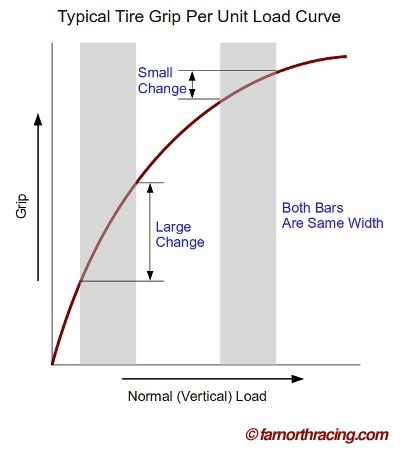
\includegraphics[width=1.0\columnwidth]{images-dis12/tire_load_curve} \\
    tire grip curve
  \end{figure}
\end{columns}
\end{frame}

%---------------------------------------------------------------------
\section{Mechanical Tuning} % [?? mins]
%---------------------------------------------------------------------
\begin{frame}
\centering \huge Mechanical Tuning
\end{frame}

%---------------------------------------------------------------------
\subsection{Suspension Tuning}

\begin{frame}
\frametitle{Camber}
\begin{columns}[t]
\column{0.646\textwidth}
  Camber: angle between wheel and vertical (from front)
  \begin{itemize}
    \item Positive if tilting outwards
    \item Negative if tilting inwards
  \end{itemize}
  \vspace{\baselineskip}
  What's optimal to maximize contact area?
  \visible<2-> {
  \begin{itemize}
    \item 0 degree, ideally
  \end{itemize}
  \vspace{\baselineskip}
  But need to account for turning chassis roll
  }
  \visible<3-> {
  \begin{itemize}
    \item Increases camber angle during turns
    \item So slightly negative camber (1\textdegree-4\textdegree) to increase traction when cornering
  \end{itemize}
  }
\column{0.323\textwidth}
  \begin{figure}
    \centering
    \only<1> {
    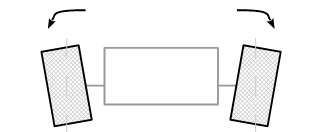
\includegraphics[scale=0.3]{images-dis12/car-camber-pos} \\
    positive camber \\
    \vspace{\baselineskip}
    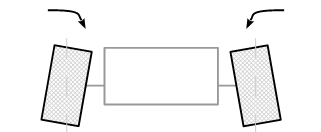
\includegraphics[scale=0.3]{images-dis12/car-camber-neg} \\
    negative camber
    }
    \visible<2-> {
    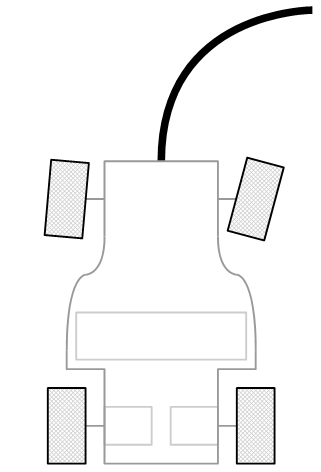
\includegraphics[scale=0.3]{images-dis12/car-top-turning} \\
    }
    \visible<4-> {
    \vspace{\baselineskip}
    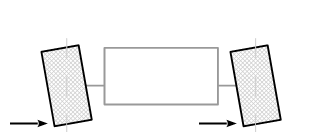
\includegraphics[scale=0.3]{images-dis12/car-camber-deform} \\
    camber effects from turning
    }
  \end{figure}
\end{columns}
\end{frame}

\begin{frame}
\frametitle{Caster}
\begin{columns}[t]
\column{0.646\textwidth}
  Caster: angle between steering axis and vertical
  \begin{itemize}
    \item Positive when steering axis line intersects road ahead of contact patch
  \end{itemize}
  \vspace{\baselineskip}
  What are the stability effects of positive caster?
  {\scriptsize think shopping cart ``caster'' wheels}
  \visible<2-> {
  \begin{itemize}  
    \item Self-centering effect
    \begin{itemize}
      \item Contact patch ``trails'' steering axis
    \end{itemize}
    \item Typically 3\textdegree-5\textdegree recommended
    \begin{itemize}
      \item Less may increase steering at stability cost
    \end{itemize}
    \item Overall effect is fairly small
  \end{itemize}
  }
\column{0.323\textwidth}
  \begin{figure}
    \centering
    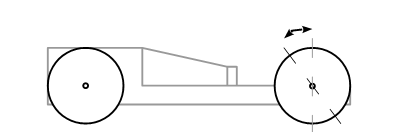
\includegraphics[scale=0.3]{images-dis12/car-side-caster} \\
    caster \\
    \vspace{\baselineskip}
    \visible<2> {
    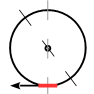
\includegraphics[scale=0.3]{images-dis12/caster-contact} \\
    self-centering effect
    }
  \end{figure}
\end{columns}
\end{frame}

\begin{frame}
\frametitle{Toe}
\begin{columns}[t]
\column{0.646\textwidth}
  Toe: angle between wheels, viewed from top
  \begin{itemize}
    \item Toe-in (positive): inwards towards front
    \item Toe-out (negative): outwards towards front
  \end{itemize}
  \vspace{\baselineskip}
  Effects of toe:
  \begin{itemize}
    \item Toe-in provides straight-line stability
    \item Toe-out provides better turn-in but amplifies disturbances
    \item Small changes produces noticable effect
    \item Recommended range (front): -3\textdegree-1\textdegree
  \end{itemize}  
  \vspace{\baselineskip}
  Why might toe be bad?
  \visible<2->{
  \begin{itemize}
    \item Wheels rub against road - reduces tire life
  \end{itemize}
  }
\column{0.323\textwidth}
  \begin{figure}
    \centering
    \vspace{-1.5\baselineskip}
    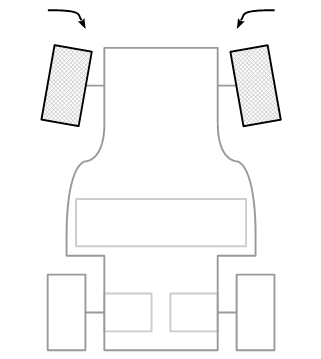
\includegraphics[scale=0.3]{images-dis12/car-top-toe-in} \\
    toe-in \\
    \vspace{\baselineskip}
    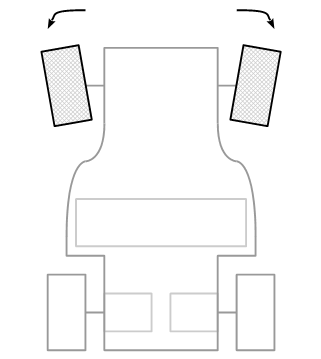
\includegraphics[scale=0.3]{images-dis12/car-top-toe-out} \\    
    toe-out
  \end{figure}
\end{columns}
\end{frame}

%---------------------------------------------------------------------
\subsection{Weight Tuning}

\begin{frame}
\frametitle{Weight Distribution}
\begin{columns}[t]
\column{0.646\textwidth}
  Freescale Car setup:
  \begin{itemize}
    \item Front wheels: steering
    \item Rear wheels: power
  \end{itemize}
  \vspace{\baselineskip}
  What does front/back weight distribution do?
  \visible<2-> {
  \begin{itemize}
    \item Towards front: more steering grip
    \item Towards back: more acceleration traction
  \end{itemize}
  }
\column{0.323\textwidth}
  \begin{figure}
    \centering
    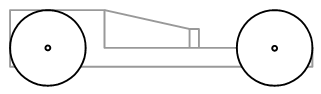
\includegraphics[scale=0.3]{images-dis12/car-side} \\
  \end{figure}
\end{columns}
\end{frame}

%---------------------------------------------------------------------
\section{Vehicle Dynamics} % [?? mins]
%---------------------------------------------------------------------
\begin{frame}
\centering \huge Vehicle Dynamics
\end{frame}

%---------------------------------------------------------------------
\subsection{Weight Transfer}

\begin{frame}
\frametitle{Lateral Weight Transfer}
\begin{columns}[t]
\column{0.646\textwidth}
  What happens to my effective weight distribution when turning? \\
  {\scriptsize assume stiff suspension for simplicity} \\
  {\scriptsize analysis with springs much more involved}
  \visible<2-> {
  \begin{itemize}
    \item Inward turning force from wheels
    \item Applies torque, rolling to outer side of turn
    \item Increases pressure on outer wheel
    \item Decreases pressure on inner wheel
  \end{itemize}
  \vspace{\baselineskip}
  So total grip reduced - how to fix?
  }
  \visible<3-> {
  \begin{itemize}
    \item Note lever effect of turning force
    \item Shorten lever to reduce torque
  \end{itemize}
  }
\column{0.323\textwidth}
  \begin{figure}
    \centering
    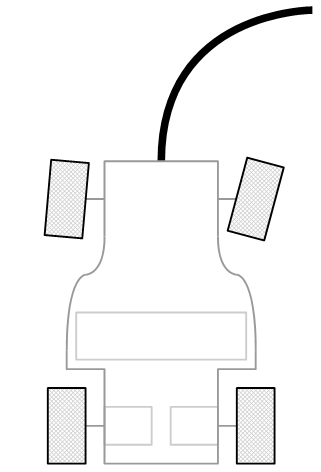
\includegraphics[scale=0.3]{images-dis12/car-top-turning} \\
    direction of travel \\
    \vspace{\baselineskip}
    \visible<2-> {
    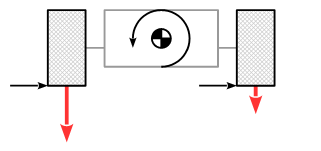
\includegraphics[scale=0.3]{images-dis12/car-weighttransfer-lateral-fbd} \\
    weight transfer
    }
  \end{figure}
\end{columns}
\end{frame}

\begin{frame}
\frametitle{Longitudal Weight Transfer}
\begin{columns}[t]
\column{0.646\textwidth}
  What happens to my effective weight distribution when accelerating?
  \visible<2-> {
  \begin{itemize}
    \item Acceleration force produced at rear wheel
    \item Applies torque pitching up
    \item Increases traction on motor wheels
    \item Decreases grip on steering wheels
  \end{itemize}
  }
\column{0.323\textwidth}
  \begin{figure}
    \centering
    \visible<2-> {
    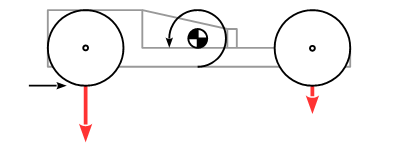
\includegraphics[scale=0.3]{images-dis12/car-weighttransfer-longitudal-fbd}
    }
  \end{figure}
\end{columns}
\end{frame}

\begin{frame}
\frametitle{Tuning Ride Height}
\begin{columns}[t]
\column{0.646\textwidth}
  Ride height: distance between track surface to underside of chassis \\
  \vspace{\baselineskip}
  We know lower center-of-gravity minimizes weight transfer. What are the limits?
  \visible<2-> {
  \begin{itemize}
    \item Need to clear uneven surfaces
    \begin{itemize}
      \item Like the courtyard tile gaps
      \item Or the Freescale Cup hump
    \end{itemize}
    \item Don't drag your chassis
    \begin{itemize}
      \item \textit{you know who you are...}
    \end{itemize}
  \end{itemize}
  }
\column{0.323\textwidth}
  \begin{figure}
    \centering
    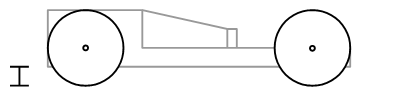
\includegraphics[width=1.0\columnwidth]{images-dis12/car-side-rideheight} \\
    ride height
  \end{figure}
\end{columns}
\end{frame}

%---------------------------------------------------------------------
\subsection{Steering}

\begin{frame}
\frametitle{Ackermann Steering}
\begin{columns}[t]
\column{0.646\textwidth}
  You may have noticed that your wheels aren't parallel when turning. Why?
  \visible<2-> {
  \begin{itemize}
    \item Different turn radius for inner/outer wheels
    \item Ackermann steering: angular difference between inner and outer wheels for different turn radius
    \item A result of the different lengths / angles of steering linkages
  \end{itemize}
  }
\column{0.323\textwidth}
  \begin{figure}
    \centering
    \only<1> {
    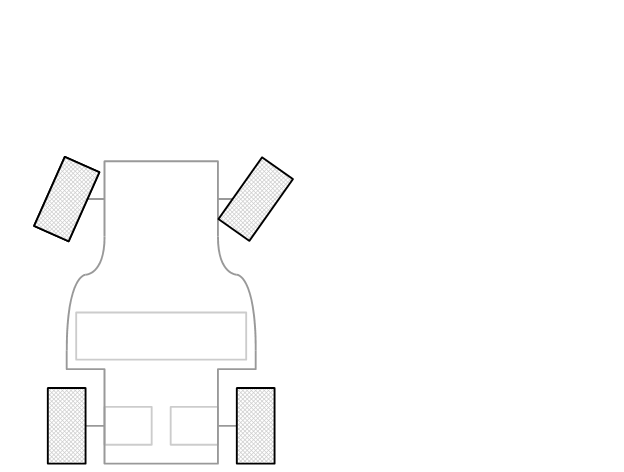
\includegraphics[width=1.0\columnwidth]{images-dis12/car-top-ackermann-nomarkings} \\
    }
    \only<2> {
    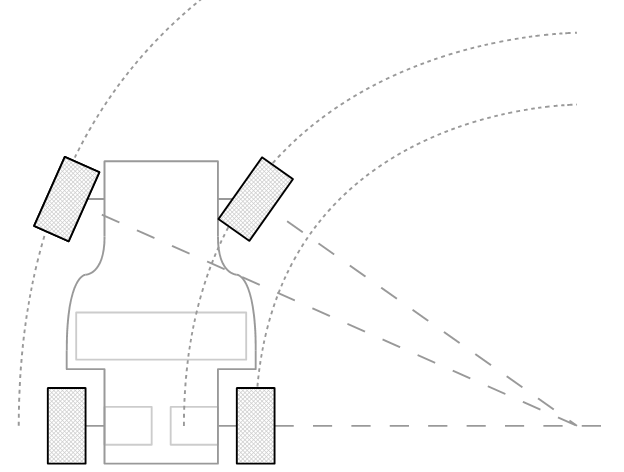
\includegraphics[width=1.0\columnwidth]{images-dis12/car-top-ackermann} \\
    }
  \end{figure}
\end{columns}
\end{frame}

\begin{frame}
\frametitle{Slipping}
\begin{columns}[t]
\column{0.646\textwidth}
  Given the Ackermann steering geometry... \\
  \vspace{2\baselineskip}
  What happens if the front wheels slip?
  \visible<2-> {
  \begin{itemize}
    \item Understeer: turns less than intended
    \item Turning radius increased
  \end{itemize}
  \vspace{\baselineskip}
  What happens if the back wheels slip?
  }
  \visible<3-> {
  \begin{itemize}
    \item Oversteer: turns more than intended
    \item Turning radius decreased
  \end{itemize}
  }
\column{0.323\textwidth}
  \begin{figure}
    \centering
    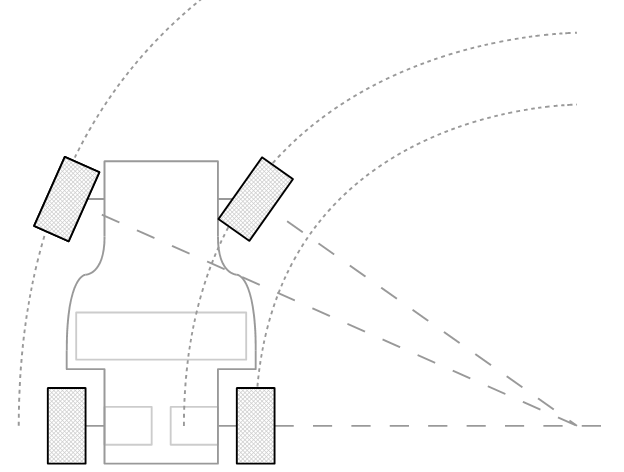
\includegraphics[width=1.0\columnwidth]{images-dis12/car-top-ackermann} \\
    % TODO: oversteering / understeering illustrations
  \end{figure}
\end{columns}
\end{frame}

\begin{frame}
\frametitle{Benchmarking}
\begin{columns}[t]
\column{0.646\textwidth}
  Obviously, what matters in the end is measurable performance \\
  \vspace{\baselineskip}
  So, what are some ways to measure success?
  \visible<2-> {
  \begin{itemize}
    \item Straight-line acceleration
    \item Maximum cornering velocity
    \item Minimum cornering radius
  \end{itemize}
  \vspace{\baselineskip}
  We've typically had less experience with mechanical tuning
  \begin{itemize}
    \item Try to benchmark and measure results
    \item Have a known-good configuration
    \begin{itemize}
      \item ``The better is the enemy of the good''
    \end{itemize}
    \item Sensor and control algorithms important
  \end{itemize}
  }
\column{0.323\textwidth}
  \begin{figure}
    \centering
    % TODO: something here?
  \end{figure}
\end{columns}
\end{frame}

%---------------------------------------------------------------------
\section*{Summary} % [?? mins]

\begin{frame}
\frametitle{Summary}
Summary
\begin{itemize}
  \item \textbf{Demo:} adjusting suspension parameters
  \item Maximize grip to maximize acceleration to reduce track times
  \item Tune camber (slightly negative), caster (slightly positive), toe
  \item Lower center of gravity: minimize weight transfer
  \item Measure, measure, measure
  % TODO: REFERENCES
  \vspace{\baselineskip}
  \item Many topics not covered: tires, springs, shocks, sprung roll
\end{itemize}
  \vspace{\baselineskip}
  \vspace{\baselineskip}
(Possibly) one more discussion section left
\begin{itemize}
  \item Any topics people want to see?
\end{itemize}
\end{frame}

\end{document}
